%META {"question":"Trên hình có bốn tia Ox, Oy, Oz, Ot chung gốc O, trong đó không có tia nào là tia đối của tia nào. Trên hình có tất cả bao nhiêu góc (không kể góc bẹt)?","options":["4 góc","5 góc","6 góc","8 góc"],"answer":2,"note":"Mỗi cặp tia cho đúng một góc. Chọn 2 trong 4 tia: 4 × 3 : 2 = 6 góc: xOy, xOz, xOt, yOz, yOt, zOt."}
\documentclass[border=5pt]{standalone}
\usepackage{tkz-euclide}
% Màu dùng chung cho toàn bộ hình vẽ (ảnh stack với nền tối của web)
\definecolor{tminc}{RGB}{226,232,240}   % chữ + nét chính
\definecolor{tmblue}{RGB}{0,210,255}    % nhấn neon xanh
\definecolor{tmpink}{RGB}{255,0,200}    % nhấn neon hồng
\definecolor{tmgreen}{RGB}{0,255,136}   % nhấn neon xanh lá
\color{tminc}

\begin{document}
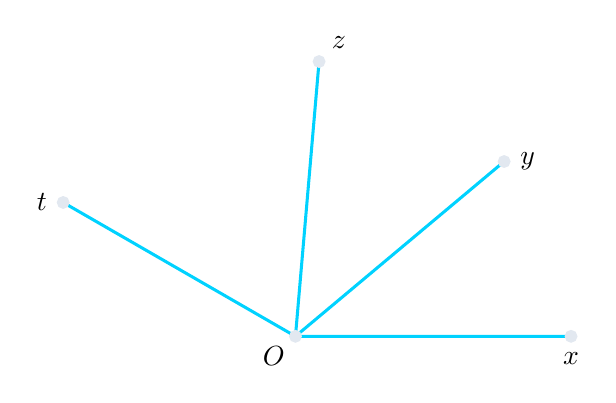
\begin{tikzpicture}[line width=1.1pt]
  \coordinate (O) at (0,0);
  \coordinate (A) at (3.5,0);
  \coordinate (B) at (2.65,2.22);
  \coordinate (C) at (0.3,3.49);
  \coordinate (D) at (-2.95,1.7);
  \draw[tmblue] (O) -- (A) (O) -- (B) (O) -- (C) (O) -- (D);
  \tkzDrawPoints[size=3.5,color=tminc,fill=tminc](O,A,B,C,D)
  \tkzLabelPoint[below left](O){$O$}
  \tkzLabelPoint[below=2pt](A){$x$}
  \tkzLabelPoint[right=2pt](B){$y$}
  \tkzLabelPoint[above right=1pt](C){$z$}
  \tkzLabelPoint[left=2pt](D){$t$}
\end{tikzpicture}
\end{document}
